\documentclass[a4paper, 14pt]{extarticle}
\usepackage[settings]{markdown}
\usepackage{minted}

% Поля
%--------------------------------------
\usepackage{geometry}
\geometry{a4paper,tmargin=2cm,bmargin=2cm,lmargin=3cm,rmargin=1cm}
%--------------------------------------


%Russian-specific packages
%--------------------------------------
\usepackage[T2A]{fontenc}
\usepackage[utf8]{inputenc} 
\usepackage[english, main=russian]{babel}
%--------------------------------------

\usepackage{textcomp}

% Красная строка
%--------------------------------------
\usepackage{indentfirst}               
%--------------------------------------             


%Graphics
%--------------------------------------
\usepackage{graphicx}
\graphicspath{ {./images/} }
\usepackage{wrapfig}
%--------------------------------------

% Полуторный интервал
%--------------------------------------
\linespread{1.3}                    
%--------------------------------------

%Выравнивание и переносы
%--------------------------------------
% Избавляемся от переполнений
\sloppy
% Запрещаем разрыв страницы после первой строки абзаца
\clubpenalty=10000
% Запрещаем разрыв страницы после последней строки абзаца
\widowpenalty=10000
%--------------------------------------

%Списки
\usepackage{enumitem}

%Подписи
\usepackage{caption} 

%Гиперссылки
\usepackage{hyperref}

\hypersetup {
	unicode=true
}

%Рисунки
%--------------------------------------
\DeclareCaptionLabelSeparator*{emdash}{~--- }
\captionsetup[figure]{labelsep=emdash,font=onehalfspacing,position=bottom}
%--------------------------------------

\usepackage{tempora}
\usepackage{amsmath}
\usepackage{color}
\usepackage{listings}
\lstset{
  belowcaptionskip=1\baselineskip,
  breaklines=true,
  frame=L,
  xleftmargin=\parindent,
  language=Python,
  showstringspaces=false,
  basicstyle=\footnotesize\ttfamily,
  keywordstyle=\bfseries\color{blue},
  commentstyle=\itshape\color{purple},
  identifierstyle=\color{black},
  stringstyle=\color{red},
}

%--------------------------------------
%			НАЧАЛО ДОКУМЕНТА
%--------------------------------------

\begin{document}

%--------------------------------------
%			ТИТУЛЬНЫЙ ЛИСТ
%--------------------------------------
\begin{titlepage}
\thispagestyle{empty}
\newpage


%Шапка титульного листа
%--------------------------------------
\vspace*{-60pt}
\hspace{-65pt}
\begin{minipage}{0.3\textwidth}
\hspace*{-20pt}\centering

\includegraphics[width=\textwidth]{emblem}
\end{minipage}
\begin{minipage}{0.67\textwidth}\small \textbf{
\vspace*{-0.7ex}
\hspace*{-6pt}\centerline{Министерство науки и высшего образования Российской Федерации}
\vspace*{-0.7ex}
\centerline{Федеральное государственное бюджетное образовательное учреждение }
\vspace*{-0.7ex}
\centerline{высшего образования}
\vspace*{-0.7ex}
\centerline{<<Московский государственный технический университет}
\vspace*{-0.7ex}
\centerline{имени Н.Э. Баумана}
\vspace*{-0.7ex}
\centerline{(национальный исследовательский университет)>>}
\vspace*{-0.7ex}
\centerline{(МГТУ им. Н.Э. Баумана)}}
\end{minipage}
%--------------------------------------

%Полосы
%--------------------------------------
\vspace{-25pt}
\hspace{-35pt}\rule{\textwidth}{2.3pt}

\vspace*{-20.3pt}
\hspace{-35pt}\rule{\textwidth}{0.4pt}
%--------------------------------------

\vspace{1.5ex}
\hspace{-35pt} \noindent \small ФАКУЛЬТЕТ\hspace{20pt} <<Информатика, искусственный интеллект и системы управления>>

\vspace*{-16pt}
\hspace{47pt}\rule{0.83\textwidth}{0.4pt}

\vspace{0.5ex}
\hspace{-35pt} \noindent \small КАФЕДРА\hspace{50pt} <<Прикладная математика и информатика>>

\vspace*{-16pt}
\hspace{30pt}\rule{0.866\textwidth}{0.4pt}
  
\vspace{11em}

\begin{center}
\Large {\bf Лабораторная работа № 6} \\ 
\large {\bf по курсу <<Алгоритмы компьютерной графики>>}\\
% \large <<Модельно-видовые и проективные пеобразования>>
\end{center}\normalsize

\vspace{8em}


\begin{flushright}
  {Студент группы ИУ9-41Б Горбунов А. Д.\hspace*{15pt} \\
  \vspace{2ex}
  Преподаватель Цапкович П. А.\hspace*{15pt}}
\end{flushright}

\bigskip

\vfill
 

\begin{center}
\textsl{Москва 2024}
\end{center}
\end{titlepage}
%--------------------------------------
%		КОНЕЦ ТИТУЛЬНОГО ЛИСТА
%--------------------------------------

\renewcommand{\ttdefault}{pcr}

\setlength{\tabcolsep}{3pt}
\newpage
\setcounter{page}{2}

\section{Цель}\label{Sect::task}
\par
Целью работы является знакомство с библиотекой OpenGL, принципами разработки алгоритмов копмьютерной графики и их реализацией на языке C++.
\section{Задание}\label{Sect::task}
\par
а. Базовой лабораторной работой является лабораторная работа №3 (модельно-видовые
преобразования и преобразования проецирования).

б. Определить параметры модели освещения OpenGL (свойства источника света, свойства
материалов (поверхностей), характеристики глобальной модели освещения).

в. Исследовать один из методов повышения реалистичности получаемых изображений сцены
(учет ослабления интенсивности света с расстоянием от источника).

г. Реализовать один из алгоритмов анимации (моделирование движения тела (с заданной начальной скоростью) при условии абсолютно упругого отражения объекта от границ некоторого ограничивающего объема (регулярной формы))

д. Реализовать наложение текстуры (загрузка из файла *.bmp или процедурная генерация) с возможностью отключения использование текстуры для определения свойств поверхности (модулирование коэффициента диффузного отражения)
\pagebreak
\section{Практическая реализация}
\begin{minted}{C++}
#include <GLFW/glfw3.h>
#include <cmath>
#define STB_IMAGE_IMPLEMENTATION
#include "stb_image.h"
#include "iostream"
using std::cos, std::sin;
int mode = 1;
int lightMode = 1;
int degreeMode = 1;
int timeMode = 0;
float degree_y = 0.0;   
float degree_x = 0.0;
float move_y = 0.0;
float move_x = 0.0;
float osnov_x = 0.1;
float osnov_y = 0.0;
float flying_speed = 0;
float V = 3.14 * pow(10,-4);
float acl = pow(10,-4);
int width = 1000;
int height = 1000;
GLuint textureID;
void key_callback(GLFWwindow *window, int key, int scancode, int action, int mods)
{
    if (action == GLFW_PRESS || action == GLFW_REPEAT)
    {
        if (key == GLFW_KEY_ESCAPE)
        {
            glfwSetWindowShouldClose(window, GL_TRUE);
        }
        else if (key == GLFW_KEY_UP)
        {
            degree_y += 0.2;
        }
        else if (key == GLFW_KEY_DOWN)
        {
            degree_y -= 0.2;
        }
        else if (key == GLFW_KEY_LEFT)
        {
            degree_x += 0.2;
        }
        else if (key == GLFW_KEY_RIGHT)
        {
            degree_x -= 0.2;
        }
        else if (key == GLFW_KEY_D)
        {
            move_x += 0.2;
        }
        else if (key == GLFW_KEY_A)
        {
            move_x -= 0.2;
        }
        else if (key == GLFW_KEY_W)
        {
            move_y += 0.2;
        }
        else if (key == GLFW_KEY_S)
        {
            move_y -= 0.2;
        }
        else if (key == GLFW_KEY_L)
        {
            osnov_x += 0.1;
        }
        else if (key == GLFW_KEY_K)
        {
            osnov_x -= 0.1;
        }
        else if (key == GLFW_KEY_I)
        {
            osnov_y += 0.1;
        }
        else if (key == GLFW_KEY_O)
        {
            osnov_y -= 0.1;
        }
        else if (key == GLFW_KEY_SPACE) 
        {
            mode = (mode + 1) % 2;
            if (mode == 0)
                glPolygonMode(GL_FRONT_AND_BACK, GL_LINE);
            else 
                glPolygonMode(GL_FRONT_AND_BACK, GL_FILL);
            
        }
        else if (key == GLFW_KEY_1)
        {
            lightMode = (lightMode + 1) % 2;
            glDisable(GL_LIGHT0);
        }
        else if (key == GLFW_KEY_2)
        {
            degreeMode = (degreeMode + 1) % 2;
        }
        else if (key == GLFW_KEY_3)
        {
            timeMode = (timeMode + 1) % 2;
        }
    }
}
void light()
{
    glPushMatrix();
    glLoadIdentity();
    glTranslatef(1, 1, 1);
    GLfloat material_diffuse[] = {0.75, 0.75, 0.75, 0.0};
    glMaterialfv(GL_FRONT_AND_BACK, GL_DIFFUSE, material_diffuse);
    GLfloat light2_diffuse[] = {1, 1, 1};
    GLfloat light2_position[] = {0, 0, 0, 1.0};
    glEnable(GL_LIGHT0);
    glLightfv(GL_LIGHT0, GL_DIFFUSE, light2_diffuse);
    glLightfv(GL_LIGHT0, GL_POSITION, light2_position);
    glLightf(GL_LIGHT0, GL_CONSTANT_ATTENUATION, 0.0);
    glLightf(GL_LIGHT0, GL_LINEAR_ATTENUATION, 0.2);
    glLightf(GL_LIGHT0, GL_QUADRATIC_ATTENUATION, 0.4);
    glPopMatrix();
}
void texture()
{
    int width_1, height_1, channels;
    unsigned char* image = stbi_load("./../texture.bmp", &width_1, &height_1, &channels, 0);
    glEnable(GL_TEXTURE_2D);
    glGenTextures(1, &textureID);
    glBindTexture(GL_TEXTURE_2D, textureID);
    glTexParameterf(GL_TEXTURE_2D, GL_TEXTURE_WRAP_S, GL_REPEAT);
    glTexParameterf(GL_TEXTURE_2D, GL_TEXTURE_WRAP_T, GL_REPEAT);
    glTexParameterf(GL_TEXTURE_2D, GL_TEXTURE_MAG_FILTER, GL_NEAREST);
    glTexParameterf(GL_TEXTURE_2D, GL_TEXTURE_MIN_FILTER, GL_NEAREST);
    if (image){
        glTexImage2D(GL_TEXTURE_2D, 0, GL_RGB, width_1, height_1, 0, GL_RGB, GL_UNSIGNED_BYTE, image);
        std::cout << "1 " << std::endl;
    }
    std::cout << "2 " << std::endl;
    stbi_image_free(image);
}
void move_object()
{
    flying_speed -= V;
    V += acl;
    if(flying_speed < -2.2 or flying_speed > 2.2)
        V = -V;
}
void display(GLFWwindow* window)
{
    glClearColor (0.3, 0.3, 0.3, 0.0);
    glEnable(GL_DEPTH_TEST);
    glClear(GL_COLOR_BUFFER_BIT | GL_DEPTH_BUFFER_BIT);
    glBindTexture(GL_TEXTURE_2D, textureID);
    glPushMatrix();
    glTranslatef(0.0f + move_x, 0.0f + move_y + flying_speed, 0.0f);
    glRotatef(degree_y * 50.f, 1.f, 0.f, 0.f);
    glRotatef(degree_x * 50.f, 0.f, 1.f, 0.f);
    glBegin(GL_QUAD_STRIP);
    glColor3f(0.4f, 0.4f, 1.0f);
    for (int i = 0; i <= 360; i += 10)
    {
        float angle = i * M_PI / 180 ;
        glTexCoord2f(1 * cos(angle) + osnov_x, 0.5 * sin(angle) + osnov_y);
        glVertex3f(1 * cos(angle) + osnov_x, 0.5 * sin(angle) + osnov_y, 0.0);
        glTexCoord2f(1 * cos(angle), 0.5 * sin(angle));
        glVertex3f(1 * cos(angle), 0.5 * sin(angle), 1);
    }
    glEnd();
    glBegin(GL_POLYGON);
    glNormal3f(1, 1, -1);
    glColor3f(1.0f, 0.3f, 0.3f);
    for (int i = 0; i <= 360; i++)
    {
        float angle = i * M_PI / 180;
        glTexCoord2f(1 * cos(angle) + osnov_x, 0.5 * sin(angle) + osnov_y);
        glVertex3f(1 * cos(angle) + osnov_x, 0.5 * sin(angle) + osnov_y, 0.0);
    }
    glEnd();
    glBegin(GL_POLYGON);
    glNormal3f(1, 1, 1);
    glColor3f(0.5f, 0.7f, 0.7f);
    for (int i = 0; i <= 360; i++)
    {
        float angle = i * M_PI / 180;
        glTexCoord2f(1 * cos(angle), 0.5 * sin(angle));
        glVertex3f(1 * cos(angle), 0.5 * sin(angle), 1);
    }
    glEnd();
    glPopMatrix();
    GLfloat spec[] = {1, 1, 1, 1};
    GLfloat emiss[] = {0, 0, 0, 1};
    GLfloat shin = 50;
    glColorMaterial(GL_FRONT_AND_BACK, GL_AMBIENT_AND_DIFFUSE);
    glMaterialfv(GL_FRONT_AND_BACK, GL_SPECULAR,  spec);
    glMaterialfv(GL_FRONT_AND_BACK, GL_SHININESS, &shin);
    glMaterialfv(GL_FRONT_AND_BACK, GL_EMISSION,  emiss);
}
int main()
{
    if (!glfwInit()) 
        return -1;
    GLFWwindow* window = glfwCreateWindow(width, height, "Lab 6", NULL, NULL);
    if (!window) {
        glfwTerminate();
        return -1;
    }
    glViewport(0, 0, width, height);
    glfwMakeContextCurrent(window);
    glfwSetKeyCallback(window, key_callback);
    glScalef(0.25,0.25, 0.25);
    glEnable(GL_LIGHTING);
    glLightModelf(GL_LIGHT_MODEL_TWO_SIDE, GL_TRUE);
    glEnable(GL_NORMALIZE);
    glPolygonMode(GL_FRONT_AND_BACK, GL_FILL);
    texture();
    while (!glfwWindowShouldClose(window))
    {
        display(window);
        if(degreeMode)
            degree_x += 0.01;
        if(timeMode)
            move_object();
        if(lightMode)
            light();
        glfwSwapBuffers(window);
        glfwPollEvents();
    }
    glfwTerminate();
    return 0;
}
\end{minted}

\section{Вывод}

В данной работе я изучил возможности языка С++ в работе с библиотекой OpenGL, приобрёл навыки разработки на языке С++ алгоритмов копьютерной графики, углубил свои знания в алгоритмах способствующих построению реалистичных изображений. 

\section{Результат запуска}
    
\begin{figure}[!htb]
	\centering
	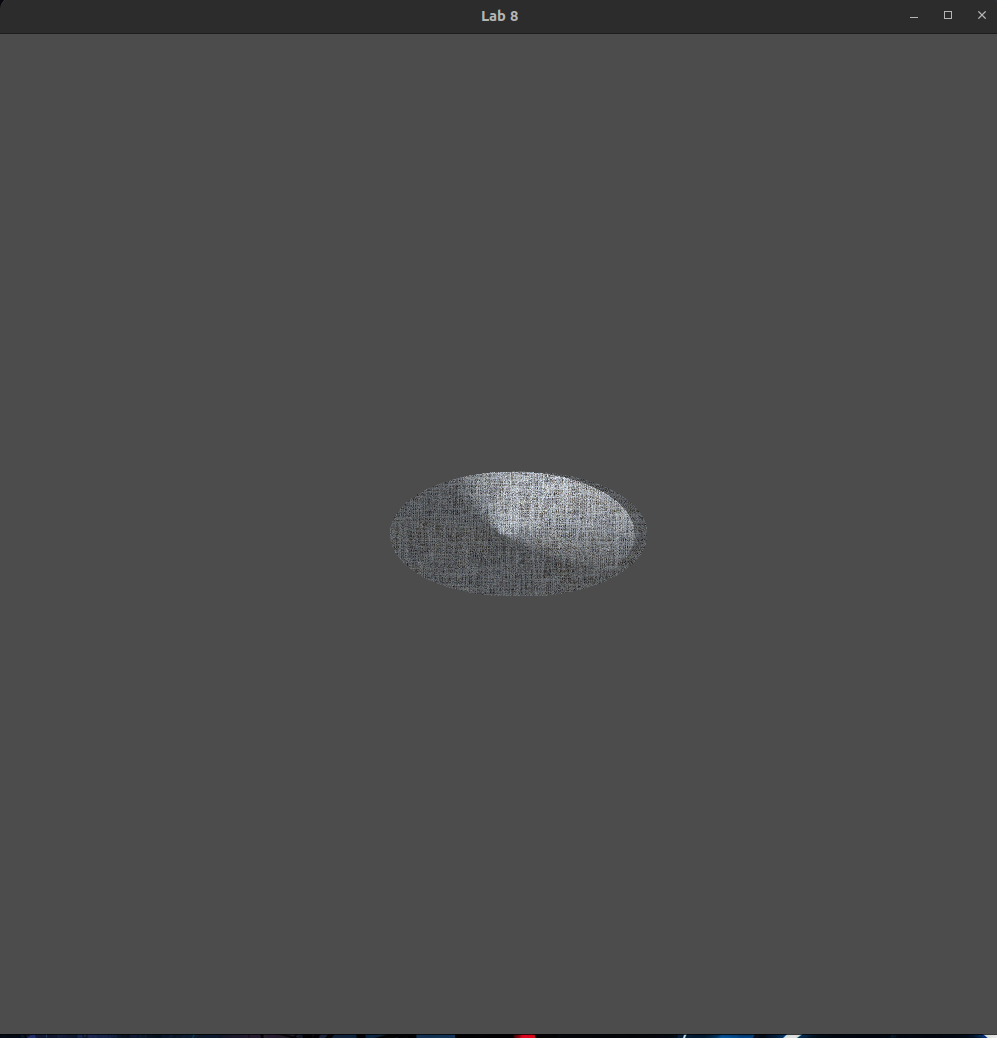
\includegraphics[width=0.8\textwidth]{picture_1.png}
\caption{ОбЪект с текстурой и освещением белого цвета}
\label{fig:picture_1.png}
\end{figure}

\begin{figure}[!htb]
	\centering
	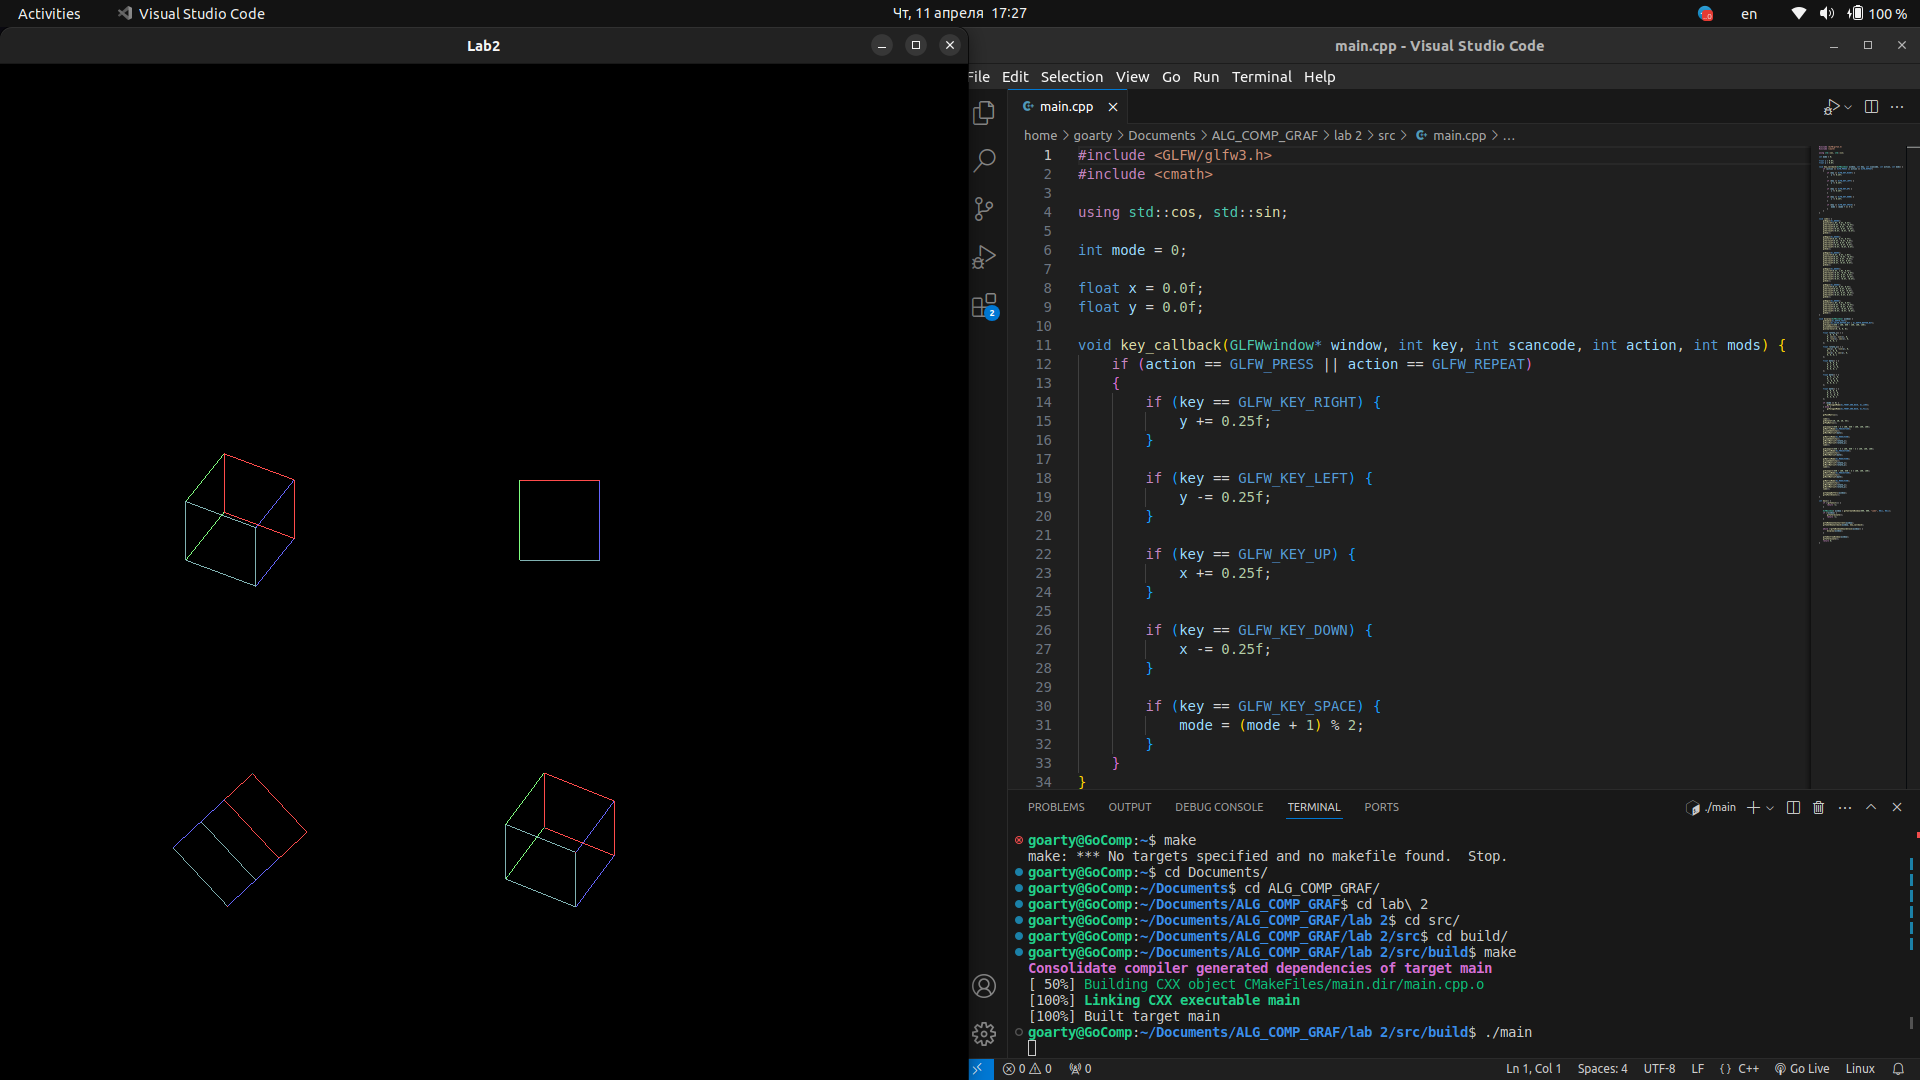
\includegraphics[width=0.8\textwidth]{picture_2.png}
\caption{ОбЪект с текстурой и освещением жёлтого цвета}
\label{fig:picture_2.png}
\end{figure}

\end{document}

